\ylDisplay{Lääts ja selle fookus} % Ülesande nimi
{Koit Timpmann} % Autor
{Lõppvoor} % Voor
{2018} % Aasta
{PK 5} % Ülesanne nr.
{2} % Raskustase
{
\ifStatement
Joonisel on kujutatud valguspunkt, sellest läätse abil saadud kujutis ning läätse optiline peatelg $O_1O_2$. Konstrueerige läätse ja selle fookuse asukohad kõikide võimalike juhtude jaoks.

%\begin{wrapfigure}{r}{0.7\textwidth}%
\vspace{-0 pt}%
\begin{center}
\includegraphics[width=0.7\linewidth]{laatsefookus.pdf}%
\end{center}
\vspace{50 pt}%
%\end{wrapfigure}	
\fi


\ifHint
Kuna pole täpsustatud kumb punktidest $A$ ja $B$ on valguspunkt ja kumb kujutis, tuleb mõlemad juhud eraldi läbi vaadata.
\fi


\ifSolution
$AB$ pikenduse ja optilise peatelje lõikepunkt vastab läätse keskpunktile. Kuna pole täpsustatud kumb punktidest on valguspunkt ja kumb kujutis, tuleb mõlemad juhud läbi vaadata.
Kui $A$ on valguspunkt ja $B$ selle kujutis, siis on tegemist kumerläätsega, mis töötab nagu luup
\vspace{-13 pt}%
\begin{center}
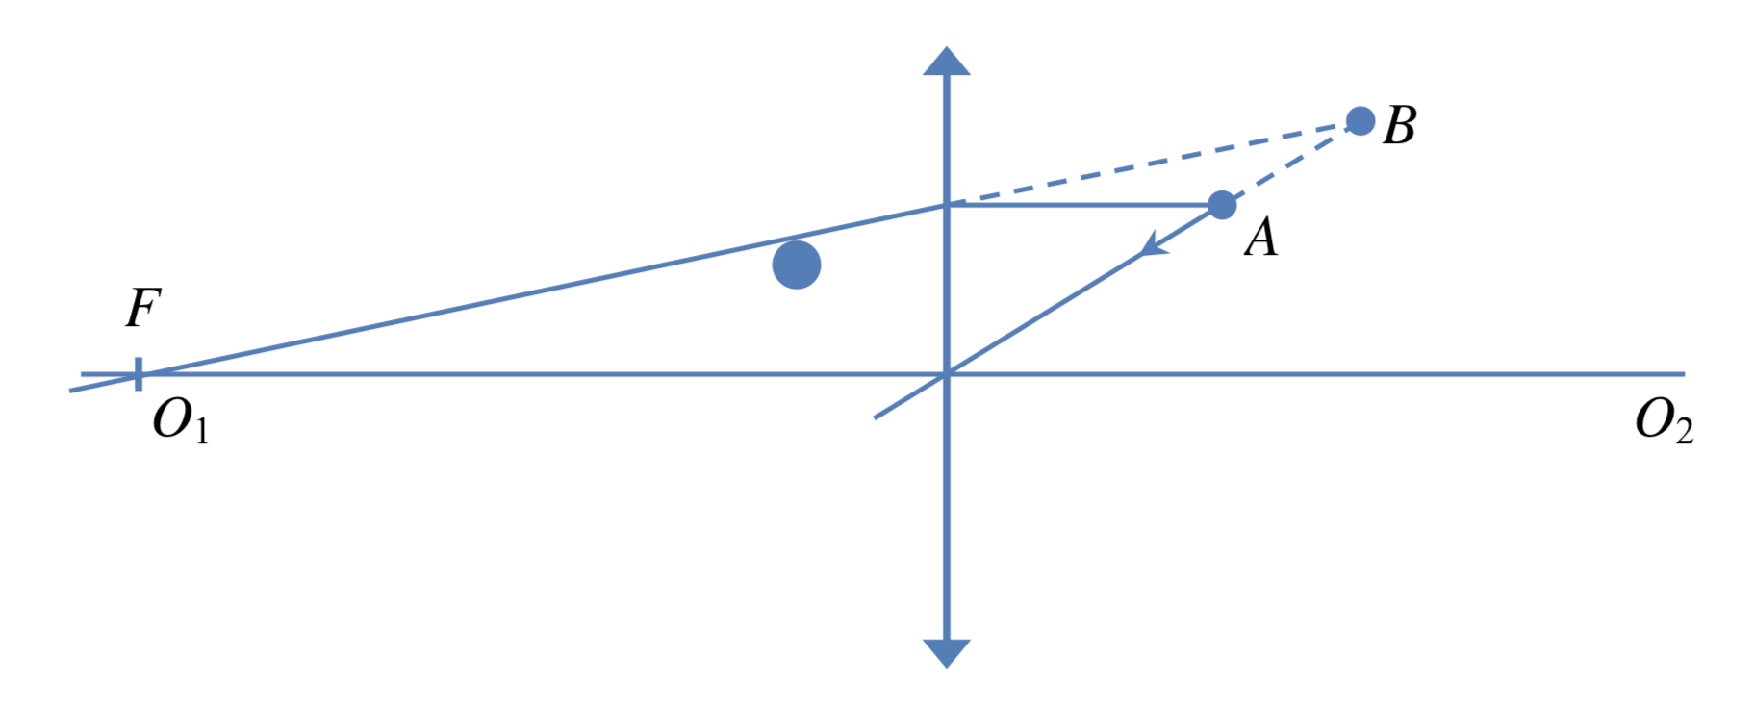
\includegraphics[angle = 270,width=0.7\linewidth]{lahenduslaats1.pdf}%
\end{center}
\vspace{-10 pt}%


Kui $A$ on valguspunkti kujutis ja $B$ valguspunkt, siis on tegemist nõgusläätsega.
\vspace{-20 pt}%
\begin{center}
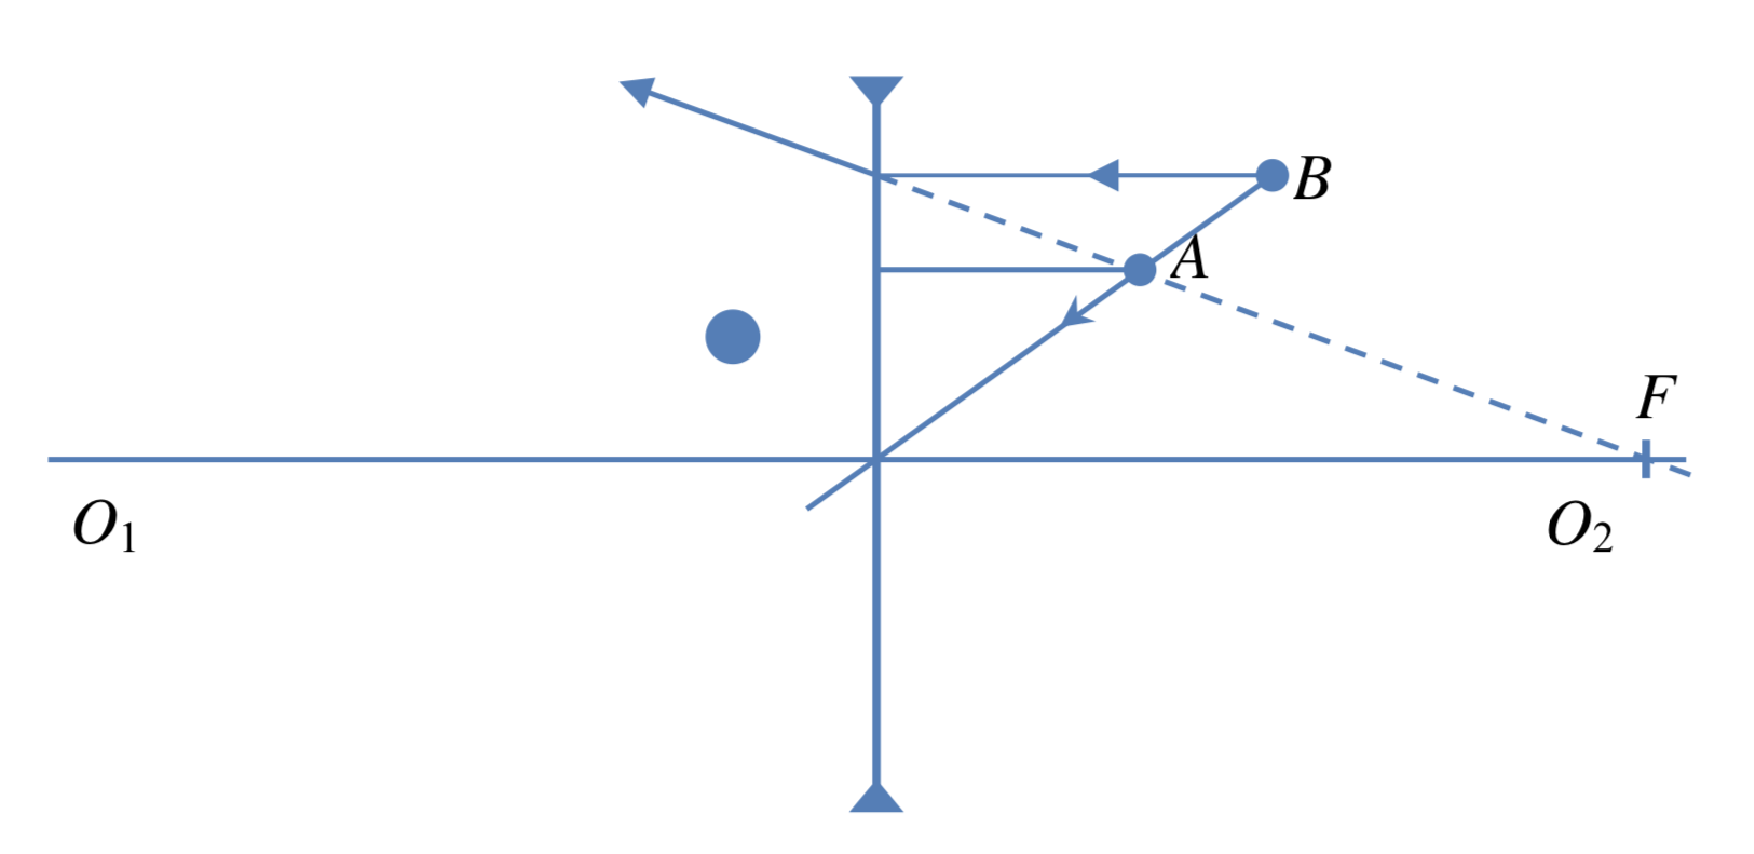
\includegraphics[angle = 270, width=0.7\linewidth]{lahenduslaats2}%
\end{center}
\vspace{-20 pt}%
\fi
}